\documentclass[12pt, twoside]{article}
\usepackage[letterpaper, margin=1in, headsep=0.5in]{geometry}
\usepackage[english]{babel}
\usepackage[utf8]{inputenc}
\usepackage{amsmath}
\usepackage{amsfonts}
\usepackage{amssymb}
\usepackage{tikz}
\usetikzlibrary{quotes, angles}
\usepackage{venndiagram}
\usepackage{multicol}

\usepackage{fancyhdr}
\pagestyle{fancy}
\fancyhf{}
\renewcommand{\headrulewidth}{0pt} % disable the underline of the header

\fancyhead[LE]{\thepage}
\fancyhead[RO]{\thepage \\ Name: \hspace{3cm}}
\fancyhead[L]{BECA / Dr. Huson / IB Math\\* 2 November 2020}


\begin{document}
\subsubsection*{2.4 Quiz: The law of sines and applications}

\begin{enumerate}

  \item Express each value as a decimal, first writing the whole calculator display, and then the 3 sig-fig approximation. \hfill [4 marks]
  \begin{multicols}{2}
    \begin{enumerate}
    \item $\displaystyle \frac{5\pi}{6}$
    \item $\displaystyle \frac{1+ \sqrt{5}}{2}$
    \end{enumerate}
  \end{multicols} \vspace{3cm}

  \item Express each value as a decimal, rounding to 3 sig-figs if necessary. \hfill [3 marks]
  \begin{multicols}{2}
    \begin{enumerate}
    \item $1.41421 \times 10^3$
    \item $1.006275 \times 10^{-2}$
    \end{enumerate}
  \end{multicols} \vspace{2cm}

  \item $\triangle ABC$ is shown with $m\angle C=90^\circ$ and the lengths of the triangle's sides are $BC=5$, $AC=12$, and $AB=13$. \vspace{1cm}
  \begin{multicols}{2}
        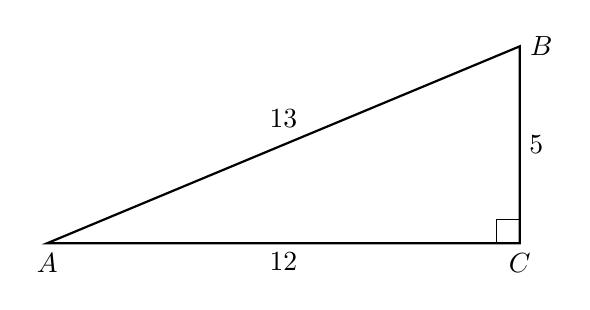
\begin{tikzpicture}[scale=0.5]
          \draw [thick]
          (0,0)node[below]{$A$}--
          (12,0)node[below]{$C$}--
          (12,5)node[right]{$B$}--cycle;
          \draw (12,0)++(-0.6,0)--++(0,0.6)--+(0.6,0);
          \node at (6,0)[below]{$12$};
          \node at (12,2.5)[right]{$5$};
          \node at (6,2.7)[above]{$13$};
        \end{tikzpicture}
        \begin{enumerate}
        \item Write down the value of $\sin A$.  \\hint: write a fraction \hfill [1 mark]\vspace{2.5cm}
        \item Find the measure of $\angle A$.  \hfill [2 marks] \vspace{1cm}
      \end{enumerate}
    \end{multicols}

\newpage
\subsubsection*{Approximations must be rounded to three significant figures and preceded by a long decimal followed by an ellipse. (e.g. $3.1415926 ...$)}
  \item Given $AB=48$, $C\hat{A}B=44^\circ$, and $A\hat{B}C=73^\circ$, as shown. Find the length of the triangle side $BC$. \hfill [4 marks]
  \begin{flushright}
    \begin{tikzpicture}[scale=1.2, rotate=20]
      \draw [-, thick] (41:4.5) node[above right]{$C$}--
        (0,0) node[left]{$A$}--
        (5,0) node[right]{$B$}--cycle;
      \node at (0.4, 0.2)[above right]{$44^\circ$};
      \node at (4.7, 0)[above left]{$73^\circ$};
      \node at (2.7, 0)[below]{$48$};
    \end{tikzpicture}
    \end{flushright}  \vspace{3cm}

    \item A ship is sailing due north. A lighthouse is sighted at a bearing of $051^\circ$ at an unknown distance, $d$. After the ship proceeds 20 kilometers, the lighthouse has a bearing of $110^\circ$. \\[0.5cm]
    Find the original distance to the lighthouse, $d$. \hfill [6 marks]

\end{enumerate}
\end{document}
